\documentclass[1p]{elsarticle_modified}
%\bibliographystyle{elsarticle-num}

%\usepackage[colorlinks]{hyperref}
%\usepackage{abbrmath_seonhwa} %\Abb, \Ascr, \Acal ,\Abf, \Afrak
\usepackage{amsfonts}
\usepackage{amssymb}
\usepackage{amsmath}
\usepackage{amsthm}
\usepackage{scalefnt}
\usepackage{amsbsy}
\usepackage{kotex}
\usepackage{caption}
\usepackage{subfig}
\usepackage{color}
\usepackage{graphicx}
\usepackage{xcolor} %% white, black, red, green, blue, cyan, magenta, yellow
\usepackage{float}
\usepackage{setspace}
\usepackage{hyperref}

\usepackage{tikz}
\usetikzlibrary{arrows}

\usepackage{multirow}
\usepackage{array} % fixed length table
\usepackage{hhline}

%%%%%%%%%%%%%%%%%%%%%
\makeatletter
\renewcommand*\env@matrix[1][\arraystretch]{%
	\edef\arraystretch{#1}%
	\hskip -\arraycolsep
	\let\@ifnextchar\new@ifnextchar
	\array{*\c@MaxMatrixCols c}}
\makeatother %https://tex.stackexchange.com/questions/14071/how-can-i-increase-the-line-spacing-in-a-matrix
%%%%%%%%%%%%%%%

\usepackage[normalem]{ulem}

\newcommand{\msout}[1]{\ifmmode\text{\sout{\ensuremath{#1}}}\else\sout{#1}\fi}
%SOURCE: \msout is \stkout macro in https://tex.stackexchange.com/questions/20609/strikeout-in-math-mode

\newcommand{\cancel}[1]{
	\ifmmode
	{\color{red}\msout{#1}}
	\else
	{\color{red}\sout{#1}}
	\fi
}

\newcommand{\add}[1]{
	{\color{blue}\uwave{#1}}
}

\newcommand{\replace}[2]{
	\ifmmode
	{\color{red}\msout{#1}}{\color{blue}\uwave{#2}}
	\else
	{\color{red}\sout{#1}}{\color{blue}\uwave{#2}}
	\fi
}

\newcommand{\Sol}{\mathcal{S}} %segment
\newcommand{\D}{D} %diagram
\newcommand{\A}{\mathcal{A}} %arc


%%%%%%%%%%%%%%%%%%%%%%%%%%%%%5 test

\def\sl{\operatorname{\textup{SL}}(2,\Cbb)}
\def\psl{\operatorname{\textup{PSL}}(2,\Cbb)}
\def\quan{\mkern 1mu \triangleright \mkern 1mu}

\theoremstyle{definition}
\newtheorem{thm}{Theorem}[section]
\newtheorem{prop}[thm]{Proposition}
\newtheorem{lem}[thm]{Lemma}
\newtheorem{ques}[thm]{Question}
\newtheorem{cor}[thm]{Corollary}
\newtheorem{defn}[thm]{Definition}
\newtheorem{exam}[thm]{Example}
\newtheorem{rmk}[thm]{Remark}
\newtheorem{alg}[thm]{Algorithm}

\newcommand{\I}{\sqrt{-1}}
\begin{document}

%\begin{frontmatter}
%
%\title{Boundary parabolic representations of knots up to 8 crossings}
%
%%% Group authors per affiliation:
%\author{Yunhi Cho} 
%\address{Department of Mathematics, University of Seoul, Seoul, Korea}
%\ead{yhcho@uos.ac.kr}
%
%
%\author{Seonhwa Kim} %\fnref{s_kim}}
%\address{Center for Geometry and Physics, Institute for Basic Science, Pohang, 37673, Korea}
%\ead{ryeona17@ibs.re.kr}
%
%\author{Hyuk Kim}
%\address{Department of Mathematical Sciences, Seoul National University, Seoul 08826, Korea}
%\ead{hyukkim@snu.ac.kr}
%
%\author{Seokbeom Yoon}
%\address{Department of Mathematical Sciences, Seoul National University, Seoul, 08826,  Korea}
%\ead{sbyoon15@snu.ac.kr}
%
%\begin{abstract}
%We find all boundary parabolic representation of knots up to 8 crossings.
%
%\end{abstract}
%\begin{keyword}
%    \MSC[2010] 57M25 
%\end{keyword}
%
%\end{frontmatter}

%\linenumbers
%\tableofcontents
%
\newcommand\colored[1]{\textcolor{white}{\rule[-0.35ex]{0.8em}{1.4ex}}\kern-0.8em\color{red} #1}%
%\newcommand\colored[1]{\textcolor{white}{ #1}\kern-2.17ex	\textcolor{white}{ #1}\kern-1.81ex	\textcolor{white}{ #1}\kern-2.15ex\color{red}#1	}

{\Large $\underline{12n_{0676}~(K12n_{0676})}$}

\setlength{\tabcolsep}{10pt}
\renewcommand{\arraystretch}{1.6}
\vspace{1cm}\begin{tabular}{m{100pt}>{\centering\arraybackslash}m{274pt}}
\multirow{5}{120pt}{
	\centering
	\includegraphics[width=112pt]{../../../GIT/diagram.site/Diagrams/png/2765_12n_0676.png}\\
\ \ \ A knot diagram\footnotemark}&
\allowdisplaybreaks
\textbf{Linearized knot diagam} \\
\cline{2-2}
 &
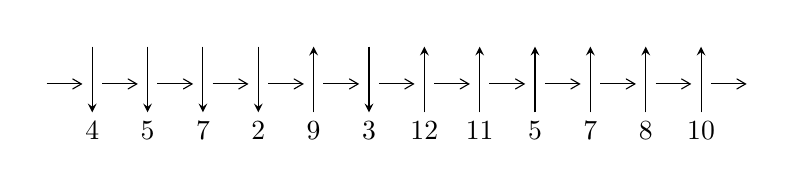
\begin{tikzpicture}[x=20pt, y=17pt]
	% nodes
	\node (C0) at (0, 0) {};
	\node (C1) at (1, 0) {};
	\node (C1U) at (1, +1) {};
	\node (C1D) at (1, -1) {4};

	\node (C2) at (2, 0) {};
	\node (C2U) at (2, +1) {};
	\node (C2D) at (2, -1) {5};

	\node (C3) at (3, 0) {};
	\node (C3U) at (3, +1) {};
	\node (C3D) at (3, -1) {7};

	\node (C4) at (4, 0) {};
	\node (C4U) at (4, +1) {};
	\node (C4D) at (4, -1) {2};

	\node (C5) at (5, 0) {};
	\node (C5U) at (5, +1) {};
	\node (C5D) at (5, -1) {9};

	\node (C6) at (6, 0) {};
	\node (C6U) at (6, +1) {};
	\node (C6D) at (6, -1) {3};

	\node (C7) at (7, 0) {};
	\node (C7U) at (7, +1) {};
	\node (C7D) at (7, -1) {12};

	\node (C8) at (8, 0) {};
	\node (C8U) at (8, +1) {};
	\node (C8D) at (8, -1) {11};

	\node (C9) at (9, 0) {};
	\node (C9U) at (9, +1) {};
	\node (C9D) at (9, -1) {5};

	\node (C10) at (10, 0) {};
	\node (C10U) at (10, +1) {};
	\node (C10D) at (10, -1) {7};

	\node (C11) at (11, 0) {};
	\node (C11U) at (11, +1) {};
	\node (C11D) at (11, -1) {8};

	\node (C12) at (12, 0) {};
	\node (C12U) at (12, +1) {};
	\node (C12D) at (12, -1) {10};
	\node (C13) at (13, 0) {};

	% arrows
	\draw[->,>={angle 60}]
	(C0) edge (C1) (C1) edge (C2) (C2) edge (C3) (C3) edge (C4) (C4) edge (C5) (C5) edge (C6) (C6) edge (C7) (C7) edge (C8) (C8) edge (C9) (C9) edge (C10) (C10) edge (C11) (C11) edge (C12) (C12) edge (C13) ;	\draw[->,>=stealth]
	(C1U) edge (C1D) (C2U) edge (C2D) (C3U) edge (C3D) (C4U) edge (C4D) (C5D) edge (C5U) (C6U) edge (C6D) (C7D) edge (C7U) (C8D) edge (C8U) (C9D) edge (C9U) (C10D) edge (C10U) (C11D) edge (C11U) (C12D) edge (C12U) ;
	\end{tikzpicture} \\
\hhline{~~} \\& 
\textbf{Solving Sequence} \\ \cline{2-2} 
 &
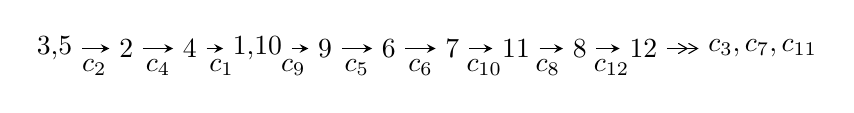
\begin{tikzpicture}[x=23pt, y=7pt]
	% node
	\node (A0) at (-1/8, 0) {3,5};
	\node (A1) at (1, 0) {2};
	\node (A2) at (2, 0) {4};
	\node (A3) at (49/16, 0) {1,10};
	\node (A4) at (33/8, 0) {9};
	\node (A5) at (41/8, 0) {6};
	\node (A6) at (49/8, 0) {7};
	\node (A7) at (57/8, 0) {11};
	\node (A8) at (65/8, 0) {8};
	\node (A9) at (73/8, 0) {12};
	\node (C1) at (1/2, -1) {$c_{2}$};
	\node (C2) at (3/2, -1) {$c_{4}$};
	\node (C3) at (5/2, -1) {$c_{1}$};
	\node (C4) at (29/8, -1) {$c_{9}$};
	\node (C5) at (37/8, -1) {$c_{5}$};
	\node (C6) at (45/8, -1) {$c_{6}$};
	\node (C7) at (53/8, -1) {$c_{10}$};
	\node (C8) at (61/8, -1) {$c_{8}$};
	\node (C9) at (69/8, -1) {$c_{12}$};
	\node (A10) at (11, 0) {$c_{3},c_{7},c_{11}$};

	% edge
	\draw[->,>=stealth]	
	(A0) edge (A1) (A1) edge (A2) (A2) edge (A3) (A3) edge (A4) (A4) edge (A5) (A5) edge (A6) (A6) edge (A7) (A7) edge (A8) (A8) edge (A9) ;
	\draw[->>,>={angle 60}]	
	(A9) edge (A10);
\end{tikzpicture} \\ 

\end{tabular} \\

\footnotetext{
The image of knot diagram is generated by the software ``\textbf{Draw programme}" developed by Andrew Bartholomew(\url{http://www.layer8.co.uk/maths/draw/index.htm\#Running-draw}), where we modified some parts for our purpose(\url{https://github.com/CATsTAILs/LinksPainter}).
}\phantom \\ \newline 
\centering \textbf{Ideals for irreducible components\footnotemark of $X_{\text{par}}$} 
 
\begin{align*}
I^u_{1}&=\langle 
-16813289 u^{16}-180512824 u^{15}+\cdots+375935808 b+173269993,\\
\phantom{I^u_{1}}&\phantom{= \langle  }296972219 u^{16}+3308940840 u^{15}+\cdots+1127807424 a-11385348987,\\
\phantom{I^u_{1}}&\phantom{= \langle  }u^{17}+11 u^{16}+\cdots-24 u+1\rangle \\
I^u_{2}&=\langle 
a^2+b+a+2,\;a^3+2 a-1,\;u-1\rangle \\
I^u_{3}&=\langle 
b^3+b^2 u+b^2-2 u-3,\;a,\;u^2+u-1\rangle \\
I^u_{4}&=\langle 
- a^3- a^2+b- a-2,\;a^4+a^3+2 a^2+2 a+1,\;u-1\rangle \\
\\
\end{align*}
\raggedright * 4 irreducible components of $\dim_{\mathbb{C}}=0$, with total 30 representations.\\
\footnotetext{All coefficients of polynomials are rational numbers. But the coefficients are sometimes approximated in decimal forms when there is not enough margin.}
\newpage
\renewcommand{\arraystretch}{1}
\centering \section*{I. $I^u_{1}= \langle -1.68\times10^{7} u^{16}-1.81\times10^{8} u^{15}+\cdots+3.76\times10^{8} b+1.73\times10^{8},\;2.97\times10^{8} u^{16}+3.31\times10^{9} u^{15}+\cdots+1.13\times10^{9} a-1.14\times10^{10},\;u^{17}+11 u^{16}+\cdots-24 u+1 \rangle$}
\flushleft \textbf{(i) Arc colorings}\\
\begin{tabular}{m{7pt} m{180pt} m{7pt} m{180pt} }
\flushright $a_{3}=$&$\begin{pmatrix}1\\0\end{pmatrix}$ \\
\flushright $a_{5}=$&$\begin{pmatrix}0\\u\end{pmatrix}$ \\
\flushright $a_{2}=$&$\begin{pmatrix}1\\- u^2\end{pmatrix}$ \\
\flushright $a_{4}=$&$\begin{pmatrix}u\\- u^3+u\end{pmatrix}$ \\
\flushright $a_{1}=$&$\begin{pmatrix}- u^2+1\\u^4-2 u^2\end{pmatrix}$ \\
\flushright $a_{10}=$&$\begin{pmatrix}-0.263318 u^{16}-2.93396 u^{15}+\cdots+47.5834 u+10.0951\\0.0447238 u^{16}+0.480169 u^{15}+\cdots-1.76545 u-0.460903\end{pmatrix}$ \\
\flushright $a_{9}=$&$\begin{pmatrix}-0.263318 u^{16}-2.93396 u^{15}+\cdots+47.5834 u+10.0951\\0.0407732 u^{16}+0.444464 u^{15}+\cdots-2.40115 u-0.423444\end{pmatrix}$ \\
\flushright $a_{6}=$&$\begin{pmatrix}-0.192384 u^{16}-2.10577 u^{15}+\cdots+12.3045 u+4.41593\\-0.00859093 u^{16}-0.0907645 u^{15}+\cdots-0.527045 u-0.177073\end{pmatrix}$ \\
\flushright $a_{7}=$&$\begin{pmatrix}-0.183793 u^{16}-2.01500 u^{15}+\cdots+12.8316 u+4.59300\\-0.00859093 u^{16}-0.0907645 u^{15}+\cdots-0.527045 u-0.177073\end{pmatrix}$ \\
\flushright $a_{11}=$&$\begin{pmatrix}-0.115128 u^{16}-1.29525 u^{15}+\cdots+24.3045 u+7.93474\\0.0334181 u^{16}+0.371617 u^{15}+\cdots-3.22037 u-0.304091\end{pmatrix}$ \\
\flushright $a_{8}=$&$\begin{pmatrix}-0.157121 u^{16}-1.73385 u^{15}+\cdots+10.9663 u+7.16044\\0.0206240 u^{16}+0.231250 u^{15}+\cdots-4.03477 u-0.167498\end{pmatrix}$ \\
\flushright $a_{12}=$&$\begin{pmatrix}0.183793 u^{16}+2.01500 u^{15}+\cdots-12.8316 u-4.59300\\-0.00282593 u^{16}-0.0405560 u^{15}+\cdots+3.13714 u+0.174058\end{pmatrix}$\\&\end{tabular}
\flushleft \textbf{(ii) Obstruction class $= -1$}\\~\\
\flushleft \textbf{(iii) Cusp Shapes $= -\frac{69994879}{187967904} u^{16}-\frac{2321600843}{563903712} u^{15}+\cdots+\frac{17938178839}{563903712} u+\frac{1576601201}{140975928}$}\\~\\
\newpage\renewcommand{\arraystretch}{1}
\flushleft \textbf{(iv) u-Polynomials at the component}\newline \\
\begin{tabular}{m{50pt}|m{274pt}}
Crossings & \hspace{64pt}u-Polynomials at each crossing \\
\hline $$\begin{aligned}c_{1},c_{2},c_{4}\end{aligned}$$&$\begin{aligned}
&u^{17}-11 u^{16}+\cdots-24 u-1
\end{aligned}$\\
\hline $$\begin{aligned}c_{3},c_{6}\end{aligned}$$&$\begin{aligned}
&u^{17}+4 u^{16}+\cdots-832 u+128
\end{aligned}$\\
\hline $$\begin{aligned}c_{5},c_{9}\end{aligned}$$&$\begin{aligned}
&u^{17}-2 u^{16}+\cdots+224 u+64
\end{aligned}$\\
\hline $$\begin{aligned}c_{7},c_{8},c_{11}\end{aligned}$$&$\begin{aligned}
&u^{17}+4 u^{16}+\cdots-6 u+1
\end{aligned}$\\
\hline $$\begin{aligned}c_{10}\end{aligned}$$&$\begin{aligned}
&u^{17}-4 u^{16}+\cdots-228 u+36
\end{aligned}$\\
\hline $$\begin{aligned}c_{12}\end{aligned}$$&$\begin{aligned}
&u^{17}+10 u^{16}+\cdots+4024 u-209
\end{aligned}$\\
\hline
\end{tabular}\\~\\
\newpage\renewcommand{\arraystretch}{1}
\flushleft \textbf{(v) Riley Polynomials at the component}\newline \\
\begin{tabular}{m{50pt}|m{274pt}}
Crossings & \hspace{64pt}Riley Polynomials at each crossing \\
\hline $$\begin{aligned}c_{1},c_{2},c_{4}\end{aligned}$$&$\begin{aligned}
&y^{17}-15 y^{16}+\cdots+798 y-1
\end{aligned}$\\
\hline $$\begin{aligned}c_{3},c_{6}\end{aligned}$$&$\begin{aligned}
&y^{17}+36 y^{16}+\cdots+487424 y-16384
\end{aligned}$\\
\hline $$\begin{aligned}c_{5},c_{9}\end{aligned}$$&$\begin{aligned}
&y^{17}-28 y^{16}+\cdots+50176 y-4096
\end{aligned}$\\
\hline $$\begin{aligned}c_{7},c_{8},c_{11}\end{aligned}$$&$\begin{aligned}
&y^{17}+14 y^{16}+\cdots+46 y-1
\end{aligned}$\\
\hline $$\begin{aligned}c_{10}\end{aligned}$$&$\begin{aligned}
&y^{17}-26 y^{16}+\cdots+52488 y-1296
\end{aligned}$\\
\hline $$\begin{aligned}c_{12}\end{aligned}$$&$\begin{aligned}
&y^{17}-42 y^{16}+\cdots+23042342 y-43681
\end{aligned}$\\
\hline
\end{tabular}\\~\\
\newpage\flushleft \textbf{(vi) Complex Volumes and Cusp Shapes}
$$\begin{array}{c|c|c}  
\text{Solutions to }I^u_{1}& \I (\text{vol} + \sqrt{-1}CS) & \text{Cusp shape}\\
 \hline 
\begin{aligned}
u &= \phantom{-}0.770740 + 0.671347 I \\
a &= -0.997689 + 0.128313 I \\
b &= \phantom{-}0.36849 + 1.84869 I\end{aligned}
 & -1.47635 + 0.05755 I & -2.53546 - 1.02432 I \\ \hline\begin{aligned}
u &= \phantom{-}0.770740 - 0.671347 I \\
a &= -0.997689 - 0.128313 I \\
b &= \phantom{-}0.36849 - 1.84869 I\end{aligned}
 & -1.47635 - 0.05755 I & -2.53546 + 1.02432 I \\ \hline\begin{aligned}
u &= \phantom{-}1.020510 + 0.262233 I \\
a &= \phantom{-}0.189037 + 0.622417 I \\
b &= \phantom{-}0.31322 + 1.67490 I\end{aligned}
 & -4.25199 + 2.42274 I & -9.52858 - 5.40161 I \\ \hline\begin{aligned}
u &= \phantom{-}1.020510 - 0.262233 I \\
a &= \phantom{-}0.189037 - 0.622417 I \\
b &= \phantom{-}0.31322 - 1.67490 I\end{aligned}
 & -4.25199 - 2.42274 I & -9.52858 + 5.40161 I \\ \hline\begin{aligned}
u &= \phantom{-}0.820811\phantom{ +0.000000I} \\
a &= -0.456752\phantom{ +0.000000I} \\
b &= \phantom{-}1.11676\phantom{ +0.000000I}\end{aligned}
 & -1.14452\phantom{ +0.000000I} & -10.7900\phantom{ +0.000000I} \\ \hline\begin{aligned}
u &= -1.51389 + 0.34866 I \\
a &= \phantom{-}0.676735 - 0.602259 I \\
b &= -0.66800 + 1.79459 I\end{aligned}
 & -11.88260 - 4.06700 I & -5.53941 + 2.68623 I \\ \hline\begin{aligned}
u &= -1.51389 - 0.34866 I \\
a &= \phantom{-}0.676735 + 0.602259 I \\
b &= -0.66800 - 1.79459 I\end{aligned}
 & -11.88260 + 4.06700 I & -5.53941 - 2.68623 I \\ \hline\begin{aligned}
u &= -0.125776 + 0.182671 I \\
a &= \phantom{-}0.73842 + 3.45151 I \\
b &= \phantom{-}0.252663 + 0.770640 I\end{aligned}
 & -3.46734 + 2.21457 I & \phantom{-}2.76869 - 2.41313 I \\ \hline\begin{aligned}
u &= -0.125776 - 0.182671 I \\
a &= \phantom{-}0.73842 - 3.45151 I \\
b &= \phantom{-}0.252663 - 0.770640 I\end{aligned}
 & -3.46734 - 2.21457 I & \phantom{-}2.76869 + 2.41313 I \\ \hline\begin{aligned}
u &= -1.87471\phantom{ +0.000000I} \\
a &= -0.672225\phantom{ +0.000000I} \\
b &= \phantom{-}2.12731\phantom{ +0.000000I}\end{aligned}
 & -7.11600\phantom{ +0.000000I} & \phantom{-}2.44290\phantom{ +0.000000I}\\
 \hline 
 \end{array}$$\newpage$$\begin{array}{c|c|c}  
\text{Solutions to }I^u_{1}& \I (\text{vol} + \sqrt{-1}CS) & \text{Cusp shape}\\
 \hline 
\begin{aligned}
u &= \phantom{-}0.0351827\phantom{ +0.000000I} \\
a &= \phantom{-}11.8728\phantom{ +0.000000I} \\
b &= -0.547681\phantom{ +0.000000I}\end{aligned}
 & \phantom{-}0.826037\phantom{ +0.000000I} & \phantom{-}12.4770\phantom{ +0.000000I} \\ \hline\begin{aligned}
u &= -1.73829 + 1.01976 I \\
a &= -0.446194 - 1.097630 I \\
b &= \phantom{-}5.09465 - 1.32883 I\end{aligned}
 & \phantom{-}7.23703 + 11.70460 I & -2.64244 - 4.71416 I \\ \hline\begin{aligned}
u &= -1.73829 - 1.01976 I \\
a &= -0.446194 + 1.097630 I \\
b &= \phantom{-}5.09465 + 1.32883 I\end{aligned}
 & \phantom{-}7.23703 - 11.70460 I & -2.64244 + 4.71416 I \\ \hline\begin{aligned}
u &= -1.85948 + 1.35841 I \\
a &= \phantom{-}0.410440 + 1.181970 I \\
b &= -6.80560 + 2.10743 I\end{aligned}
 & \phantom{-}12.6875 + 6.3547 I & \phantom{-}0.47634 - 2.59876 I \\ \hline\begin{aligned}
u &= -1.85948 - 1.35841 I \\
a &= \phantom{-}0.410440 - 1.181970 I \\
b &= -6.80560 - 2.10743 I\end{aligned}
 & \phantom{-}12.6875 - 6.3547 I & \phantom{-}0.47634 + 2.59876 I \\ \hline\begin{aligned}
u &= -1.54446 + 1.96036 I \\
a &= -0.442677 - 1.276270 I \\
b &= \phantom{-}7.09639 - 6.41609 I\end{aligned}
 & \phantom{-}9.80581 + 0.01769 I & -1.064012 + 0.845538 I \\ \hline\begin{aligned}
u &= -1.54446 - 1.96036 I \\
a &= -0.442677 + 1.276270 I \\
b &= \phantom{-}7.09639 + 6.41609 I\end{aligned}
 & \phantom{-}9.80581 - 0.01769 I & -1.064012 - 0.845538 I\\
 \hline 
 \end{array}$$\newpage\newpage\renewcommand{\arraystretch}{1}
\centering \section*{II. $I^u_{2}= \langle a^2+b+a+2,\;a^3+2 a-1,\;u-1 \rangle$}
\flushleft \textbf{(i) Arc colorings}\\
\begin{tabular}{m{7pt} m{180pt} m{7pt} m{180pt} }
\flushright $a_{3}=$&$\begin{pmatrix}1\\0\end{pmatrix}$ \\
\flushright $a_{5}=$&$\begin{pmatrix}0\\1\end{pmatrix}$ \\
\flushright $a_{2}=$&$\begin{pmatrix}1\\-1\end{pmatrix}$ \\
\flushright $a_{4}=$&$\begin{pmatrix}1\\0\end{pmatrix}$ \\
\flushright $a_{1}=$&$\begin{pmatrix}0\\-1\end{pmatrix}$ \\
\flushright $a_{10}=$&$\begin{pmatrix}a\\- a^2- a-2\end{pmatrix}$ \\
\flushright $a_{9}=$&$\begin{pmatrix}a\\- a^2-2\end{pmatrix}$ \\
\flushright $a_{6}=$&$\begin{pmatrix}a^2\\0\end{pmatrix}$ \\
\flushright $a_{7}=$&$\begin{pmatrix}a^2\\0\end{pmatrix}$ \\
\flushright $a_{11}=$&$\begin{pmatrix}- a^2- a+1\\- a^2- a-2\end{pmatrix}$ \\
\flushright $a_{8}=$&$\begin{pmatrix}a^2-2 a+1\\-1\end{pmatrix}$ \\
\flushright $a_{12}=$&$\begin{pmatrix}a^2\\- a^2-2\end{pmatrix}$\\&\end{tabular}
\flushleft \textbf{(ii) Obstruction class $= 1$}\\~\\
\flushleft \textbf{(iii) Cusp Shapes $= 11 a^2+9 a+22$}\\~\\
\newpage\renewcommand{\arraystretch}{1}
\flushleft \textbf{(iv) u-Polynomials at the component}\newline \\
\begin{tabular}{m{50pt}|m{274pt}}
Crossings & \hspace{64pt}u-Polynomials at each crossing \\
\hline $$\begin{aligned}c_{1},c_{2}\end{aligned}$$&$\begin{aligned}
&(u-1)^3
\end{aligned}$\\
\hline $$\begin{aligned}c_{3},c_{6}\end{aligned}$$&$\begin{aligned}
&u^3
\end{aligned}$\\
\hline $$\begin{aligned}c_{4}\end{aligned}$$&$\begin{aligned}
&(u+1)^3
\end{aligned}$\\
\hline $$\begin{aligned}c_{5},c_{7},c_{8}\end{aligned}$$&$\begin{aligned}
&u^3+2 u+1
\end{aligned}$\\
\hline $$\begin{aligned}c_{9},c_{11},c_{12}\end{aligned}$$&$\begin{aligned}
&u^3+2 u-1
\end{aligned}$\\
\hline $$\begin{aligned}c_{10}\end{aligned}$$&$\begin{aligned}
&u^3-3 u^2+5 u-2
\end{aligned}$\\
\hline
\end{tabular}\\~\\
\newpage\renewcommand{\arraystretch}{1}
\flushleft \textbf{(v) Riley Polynomials at the component}\newline \\
\begin{tabular}{m{50pt}|m{274pt}}
Crossings & \hspace{64pt}Riley Polynomials at each crossing \\
\hline $$\begin{aligned}c_{1},c_{2},c_{4}\end{aligned}$$&$\begin{aligned}
&(y-1)^3
\end{aligned}$\\
\hline $$\begin{aligned}c_{3},c_{6}\end{aligned}$$&$\begin{aligned}
&y^3
\end{aligned}$\\
\hline $$\begin{aligned}c_{5},c_{7},c_{8}\\c_{9},c_{11},c_{12}\end{aligned}$$&$\begin{aligned}
&y^3+4 y^2+4 y-1
\end{aligned}$\\
\hline $$\begin{aligned}c_{10}\end{aligned}$$&$\begin{aligned}
&y^3+y^2+13 y-4
\end{aligned}$\\
\hline
\end{tabular}\\~\\
\newpage\flushleft \textbf{(vi) Complex Volumes and Cusp Shapes}
$$\begin{array}{c|c|c}  
\text{Solutions to }I^u_{2}& \I (\text{vol} + \sqrt{-1}CS) & \text{Cusp shape}\\
 \hline 
\begin{aligned}
u &= \phantom{-}1.00000\phantom{ +0.000000I} \\
a &= -0.22670 + 1.46771 I \\
b &= \phantom{-}0.329484 - 0.802255 I\end{aligned}
 & -11.08570 - 5.13794 I & -3.17092 + 5.88938 I \\ \hline\begin{aligned}
u &= \phantom{-}1.00000\phantom{ +0.000000I} \\
a &= -0.22670 - 1.46771 I \\
b &= \phantom{-}0.329484 + 0.802255 I\end{aligned}
 & -11.08570 + 5.13794 I & -3.17092 - 5.88938 I \\ \hline\begin{aligned}
u &= \phantom{-}1.00000\phantom{ +0.000000I} \\
a &= \phantom{-}0.453398\phantom{ +0.000000I} \\
b &= -2.65897\phantom{ +0.000000I}\end{aligned}
 & -0.857735\phantom{ +0.000000I} & \phantom{-}28.3420\phantom{ +0.000000I}\\
 \hline 
 \end{array}$$\newpage\newpage\renewcommand{\arraystretch}{1}
\centering \section*{III. $I^u_{3}= \langle b^3+b^2 u+b^2-2 u-3,\;a,\;u^2+u-1 \rangle$}
\flushleft \textbf{(i) Arc colorings}\\
\begin{tabular}{m{7pt} m{180pt} m{7pt} m{180pt} }
\flushright $a_{3}=$&$\begin{pmatrix}1\\0\end{pmatrix}$ \\
\flushright $a_{5}=$&$\begin{pmatrix}0\\u\end{pmatrix}$ \\
\flushright $a_{2}=$&$\begin{pmatrix}1\\u-1\end{pmatrix}$ \\
\flushright $a_{4}=$&$\begin{pmatrix}u\\- u+1\end{pmatrix}$ \\
\flushright $a_{1}=$&$\begin{pmatrix}u\\- u\end{pmatrix}$ \\
\flushright $a_{10}=$&$\begin{pmatrix}0\\b\end{pmatrix}$ \\
\flushright $a_{9}=$&$\begin{pmatrix}0\\b\end{pmatrix}$ \\
\flushright $a_{6}=$&$\begin{pmatrix}0\\u\end{pmatrix}$ \\
\flushright $a_{7}=$&$\begin{pmatrix}- u\\u\end{pmatrix}$ \\
\flushright $a_{11}=$&$\begin{pmatrix}- b u+b\\b u\end{pmatrix}$ \\
\flushright $a_{8}=$&$\begin{pmatrix}2 b^2 u- b^2- u\\- b^2 u+b^2+b-1\end{pmatrix}$ \\
\flushright $a_{12}=$&$\begin{pmatrix}u\\b^2 u- u\end{pmatrix}$\\&\end{tabular}
\flushleft \textbf{(ii) Obstruction class $= 1$}\\~\\
\flushleft \textbf{(iii) Cusp Shapes $= - b^2 u-2 b^2- b u+3 b+3 u-4$}\\~\\
\newpage\renewcommand{\arraystretch}{1}
\flushleft \textbf{(iv) u-Polynomials at the component}\newline \\
\begin{tabular}{m{50pt}|m{274pt}}
Crossings & \hspace{64pt}u-Polynomials at each crossing \\
\hline $$\begin{aligned}c_{1},c_{2},c_{3}\end{aligned}$$&$\begin{aligned}
&(u^2+u-1)^3
\end{aligned}$\\
\hline $$\begin{aligned}c_{4},c_{6}\end{aligned}$$&$\begin{aligned}
&(u^2- u-1)^3
\end{aligned}$\\
\hline $$\begin{aligned}c_{5},c_{9}\end{aligned}$$&$\begin{aligned}
&u^6
\end{aligned}$\\
\hline $$\begin{aligned}c_{7},c_{8}\end{aligned}$$&$\begin{aligned}
&(u^3+u^2+2 u+1)^2
\end{aligned}$\\
\hline $$\begin{aligned}c_{10},c_{12}\end{aligned}$$&$\begin{aligned}
&(u^3+u^2-1)^2
\end{aligned}$\\
\hline $$\begin{aligned}c_{11}\end{aligned}$$&$\begin{aligned}
&(u^3- u^2+2 u-1)^2
\end{aligned}$\\
\hline
\end{tabular}\\~\\
\newpage\renewcommand{\arraystretch}{1}
\flushleft \textbf{(v) Riley Polynomials at the component}\newline \\
\begin{tabular}{m{50pt}|m{274pt}}
Crossings & \hspace{64pt}Riley Polynomials at each crossing \\
\hline $$\begin{aligned}c_{1},c_{2},c_{3}\\c_{4},c_{6}\end{aligned}$$&$\begin{aligned}
&(y^2-3 y+1)^3
\end{aligned}$\\
\hline $$\begin{aligned}c_{5},c_{9}\end{aligned}$$&$\begin{aligned}
&y^6
\end{aligned}$\\
\hline $$\begin{aligned}c_{7},c_{8},c_{11}\end{aligned}$$&$\begin{aligned}
&(y^3+3 y^2+2 y-1)^2
\end{aligned}$\\
\hline $$\begin{aligned}c_{10},c_{12}\end{aligned}$$&$\begin{aligned}
&(y^3- y^2+2 y-1)^2
\end{aligned}$\\
\hline
\end{tabular}\\~\\
\newpage\flushleft \textbf{(vi) Complex Volumes and Cusp Shapes}
$$\begin{array}{c|c|c}  
\text{Solutions to }I^u_{3}& \I (\text{vol} + \sqrt{-1}CS) & \text{Cusp shape}\\
 \hline 
\begin{aligned}
u &= \phantom{-}0.618034\phantom{ +0.000000I} \\
a &= \phantom{-0.000000 } 0 \\
b &= \phantom{-}1.22142\phantom{ +0.000000I}\end{aligned}
 & \phantom{-}0.126494\phantom{ +0.000000I} & -3.14230\phantom{ +0.000000I} \\ \hline\begin{aligned}
u &= \phantom{-}0.618034\phantom{ +0.000000I} \\
a &= \phantom{-0.000000 } 0 \\
b &= -1.41973 + 1.20521 I\end{aligned}
 & -4.01109 - 2.82812 I & -7.00182 + 11.83005 I \\ \hline\begin{aligned}
u &= \phantom{-}0.618034\phantom{ +0.000000I} \\
a &= \phantom{-0.000000 } 0 \\
b &= -1.41973 - 1.20521 I\end{aligned}
 & -4.01109 + 2.82812 I & -7.00182 - 11.83005 I \\ \hline\begin{aligned}
u &= -1.61803\phantom{ +0.000000I} \\
a &= \phantom{-0.000000 } 0 \\
b &= \phantom{-}0.542287 + 0.460350 I\end{aligned}
 & -11.90680 + 2.82812 I & -6.38118 + 1.93520 I \\ \hline\begin{aligned}
u &= -1.61803\phantom{ +0.000000I} \\
a &= \phantom{-0.000000 } 0 \\
b &= \phantom{-}0.542287 - 0.460350 I\end{aligned}
 & -11.90680 - 2.82812 I & -6.38118 - 1.93520 I \\ \hline\begin{aligned}
u &= -1.61803\phantom{ +0.000000I} \\
a &= \phantom{-0.000000 } 0 \\
b &= -0.466540\phantom{ +0.000000I}\end{aligned}
 & -7.76919\phantom{ +0.000000I} & -11.0920\phantom{ +0.000000I}\\
 \hline 
 \end{array}$$\newpage\newpage\renewcommand{\arraystretch}{1}
\centering \section*{IV. $I^u_{4}= \langle - a^3- a^2+b- a-2,\;a^4+a^3+2 a^2+2 a+1,\;u-1 \rangle$}
\flushleft \textbf{(i) Arc colorings}\\
\begin{tabular}{m{7pt} m{180pt} m{7pt} m{180pt} }
\flushright $a_{3}=$&$\begin{pmatrix}1\\0\end{pmatrix}$ \\
\flushright $a_{5}=$&$\begin{pmatrix}0\\1\end{pmatrix}$ \\
\flushright $a_{2}=$&$\begin{pmatrix}1\\-1\end{pmatrix}$ \\
\flushright $a_{4}=$&$\begin{pmatrix}1\\0\end{pmatrix}$ \\
\flushright $a_{1}=$&$\begin{pmatrix}0\\-1\end{pmatrix}$ \\
\flushright $a_{10}=$&$\begin{pmatrix}a\\a^3+a^2+a+2\end{pmatrix}$ \\
\flushright $a_{9}=$&$\begin{pmatrix}a\\a^3+a^2+2 a+2\end{pmatrix}$ \\
\flushright $a_{6}=$&$\begin{pmatrix}a^2\\0\end{pmatrix}$ \\
\flushright $a_{7}=$&$\begin{pmatrix}a^2\\0\end{pmatrix}$ \\
\flushright $a_{11}=$&$\begin{pmatrix}-1\\a^3+a^2+a+2\end{pmatrix}$ \\
\flushright $a_{8}=$&$\begin{pmatrix}- a^3- a-1\\3 a^3+a^2+5 a+3\end{pmatrix}$ \\
\flushright $a_{12}=$&$\begin{pmatrix}a^2\\- a^2-2\end{pmatrix}$\\&\end{tabular}
\flushleft \textbf{(ii) Obstruction class $= 1$}\\~\\
\flushleft \textbf{(iii) Cusp Shapes $= 4 a^3-3 a^2+4 a-4$}\\~\\
\newpage\renewcommand{\arraystretch}{1}
\flushleft \textbf{(iv) u-Polynomials at the component}\newline \\
\begin{tabular}{m{50pt}|m{274pt}}
Crossings & \hspace{64pt}u-Polynomials at each crossing \\
\hline $$\begin{aligned}c_{1},c_{2}\end{aligned}$$&$\begin{aligned}
&(u-1)^4
\end{aligned}$\\
\hline $$\begin{aligned}c_{3},c_{6}\end{aligned}$$&$\begin{aligned}
&u^4
\end{aligned}$\\
\hline $$\begin{aligned}c_{4}\end{aligned}$$&$\begin{aligned}
&(u+1)^4
\end{aligned}$\\
\hline $$\begin{aligned}c_{5},c_{7},c_{8}\end{aligned}$$&$\begin{aligned}
&u^4- u^3+2 u^2-2 u+1
\end{aligned}$\\
\hline $$\begin{aligned}c_{9},c_{11},c_{12}\end{aligned}$$&$\begin{aligned}
&u^4+u^3+2 u^2+2 u+1
\end{aligned}$\\
\hline $$\begin{aligned}c_{10}\end{aligned}$$&$\begin{aligned}
&(u^2+u+1)^2
\end{aligned}$\\
\hline
\end{tabular}\\~\\
\newpage\renewcommand{\arraystretch}{1}
\flushleft \textbf{(v) Riley Polynomials at the component}\newline \\
\begin{tabular}{m{50pt}|m{274pt}}
Crossings & \hspace{64pt}Riley Polynomials at each crossing \\
\hline $$\begin{aligned}c_{1},c_{2},c_{4}\end{aligned}$$&$\begin{aligned}
&(y-1)^4
\end{aligned}$\\
\hline $$\begin{aligned}c_{3},c_{6}\end{aligned}$$&$\begin{aligned}
&y^4
\end{aligned}$\\
\hline $$\begin{aligned}c_{5},c_{7},c_{8}\\c_{9},c_{11},c_{12}\end{aligned}$$&$\begin{aligned}
&y^4+3 y^3+2 y^2+1
\end{aligned}$\\
\hline $$\begin{aligned}c_{10}\end{aligned}$$&$\begin{aligned}
&(y^2+y+1)^2
\end{aligned}$\\
\hline
\end{tabular}\\~\\
\newpage\flushleft \textbf{(vi) Complex Volumes and Cusp Shapes}
$$\begin{array}{c|c|c}  
\text{Solutions to }I^u_{4}& \I (\text{vol} + \sqrt{-1}CS) & \text{Cusp shape}\\
 \hline 
\begin{aligned}
u &= \phantom{-}1.00000\phantom{ +0.000000I} \\
a &= -0.621744 + 0.440597 I \\
b &= \phantom{-}1.69244 + 0.31815 I\end{aligned}
 & -4.93480 - 2.02988 I & -6.57732 + 5.10773 I \\ \hline\begin{aligned}
u &= \phantom{-}1.00000\phantom{ +0.000000I} \\
a &= -0.621744 - 0.440597 I \\
b &= \phantom{-}1.69244 - 0.31815 I\end{aligned}
 & -4.93480 + 2.02988 I & -6.57732 - 5.10773 I \\ \hline\begin{aligned}
u &= \phantom{-}1.00000\phantom{ +0.000000I} \\
a &= \phantom{-}0.121744 + 1.306620 I \\
b &= -0.192440 - 0.547877 I\end{aligned}
 & -4.93480 + 2.02988 I & -0.92268 - 4.41855 I \\ \hline\begin{aligned}
u &= \phantom{-}1.00000\phantom{ +0.000000I} \\
a &= \phantom{-}0.121744 - 1.306620 I \\
b &= -0.192440 + 0.547877 I\end{aligned}
 & -4.93480 - 2.02988 I & -0.92268 + 4.41855 I\\
 \hline 
 \end{array}$$\newpage
\newpage\renewcommand{\arraystretch}{1}
\centering \section*{ V. u-Polynomials}
\begin{tabular}{m{50pt}|m{274pt}}
Crossings & \hspace{64pt}u-Polynomials at each crossing \\
\hline $$\begin{aligned}c_{1},c_{2}\end{aligned}$$&$\begin{aligned}
&((u-1)^7)(u^2+u-1)^3(u^{17}-11 u^{16}+\cdots-24 u-1)
\end{aligned}$\\
\hline $$\begin{aligned}c_{3}\end{aligned}$$&$\begin{aligned}
&u^7(u^2+u-1)^3(u^{17}+4 u^{16}+\cdots-832 u+128)
\end{aligned}$\\
\hline $$\begin{aligned}c_{4}\end{aligned}$$&$\begin{aligned}
&((u+1)^7)(u^2- u-1)^3(u^{17}-11 u^{16}+\cdots-24 u-1)
\end{aligned}$\\
\hline $$\begin{aligned}c_{5}\end{aligned}$$&$\begin{aligned}
&u^6(u^3+2 u+1)(u^4- u^3+\cdots-2 u+1)(u^{17}-2 u^{16}+\cdots+224 u+64)
\end{aligned}$\\
\hline $$\begin{aligned}c_{6}\end{aligned}$$&$\begin{aligned}
&u^7(u^2- u-1)^3(u^{17}+4 u^{16}+\cdots-832 u+128)
\end{aligned}$\\
\hline $$\begin{aligned}c_{7},c_{8}\end{aligned}$$&$\begin{aligned}
&(u^3+2 u+1)(u^3+u^2+2 u+1)^2(u^4- u^3+2 u^2-2 u+1)\\
&\cdot(u^{17}+4 u^{16}+\cdots-6 u+1)
\end{aligned}$\\
\hline $$\begin{aligned}c_{9}\end{aligned}$$&$\begin{aligned}
&u^6(u^3+2 u-1)(u^4+u^3+\cdots+2 u+1)(u^{17}-2 u^{16}+\cdots+224 u+64)
\end{aligned}$\\
\hline $$\begin{aligned}c_{10}\end{aligned}$$&$\begin{aligned}
&(u^2+u+1)^2(u^3-3 u^2+5 u-2)(u^3+u^2-1)^2\\
&\cdot(u^{17}-4 u^{16}+\cdots-228 u+36)
\end{aligned}$\\
\hline $$\begin{aligned}c_{11}\end{aligned}$$&$\begin{aligned}
&(u^3+2 u-1)(u^3- u^2+2 u-1)^2(u^4+u^3+2 u^2+2 u+1)\\
&\cdot(u^{17}+4 u^{16}+\cdots-6 u+1)
\end{aligned}$\\
\hline $$\begin{aligned}c_{12}\end{aligned}$$&$\begin{aligned}
&(u^3+2 u-1)(u^3+u^2-1)^2(u^4+u^3+2 u^2+2 u+1)\\
&\cdot(u^{17}+10 u^{16}+\cdots+4024 u-209)
\end{aligned}$\\
\hline
\end{tabular}\newpage\renewcommand{\arraystretch}{1}
\centering \section*{ VI. Riley Polynomials}
\begin{tabular}{m{50pt}|m{274pt}}
Crossings & \hspace{64pt}Riley Polynomials at each crossing \\
\hline $$\begin{aligned}c_{1},c_{2},c_{4}\end{aligned}$$&$\begin{aligned}
&((y-1)^7)(y^2-3 y+1)^3(y^{17}-15 y^{16}+\cdots+798 y-1)
\end{aligned}$\\
\hline $$\begin{aligned}c_{3},c_{6}\end{aligned}$$&$\begin{aligned}
&y^7(y^2-3 y+1)^3(y^{17}+36 y^{16}+\cdots+487424 y-16384)
\end{aligned}$\\
\hline $$\begin{aligned}c_{5},c_{9}\end{aligned}$$&$\begin{aligned}
&y^6(y^3+4 y^2+4 y-1)(y^4+3 y^3+2 y^2+1)\\
&\cdot(y^{17}-28 y^{16}+\cdots+50176 y-4096)
\end{aligned}$\\
\hline $$\begin{aligned}c_{7},c_{8},c_{11}\end{aligned}$$&$\begin{aligned}
&(y^3+3 y^2+2 y-1)^2(y^3+4 y^2+4 y-1)(y^4+3 y^3+2 y^2+1)\\
&\cdot(y^{17}+14 y^{16}+\cdots+46 y-1)
\end{aligned}$\\
\hline $$\begin{aligned}c_{10}\end{aligned}$$&$\begin{aligned}
&(y^2+y+1)^2(y^3- y^2+2 y-1)^2(y^3+y^2+13 y-4)\\
&\cdot(y^{17}-26 y^{16}+\cdots+52488 y-1296)
\end{aligned}$\\
\hline $$\begin{aligned}c_{12}\end{aligned}$$&$\begin{aligned}
&(y^3- y^2+2 y-1)^2(y^3+4 y^2+4 y-1)(y^4+3 y^3+2 y^2+1)\\
&\cdot(y^{17}-42 y^{16}+\cdots+23042342 y-43681)
\end{aligned}$\\
\hline
\end{tabular}
\vskip 2pc
\end{document}